\documentclass[11pt,class=report,crop=false]{standalone}
\usepackage[screen]{../python}

\begin{document}


%====================================================================
\chapitre{Game of life}
%====================================================================

\objectifs{The \emph{game of life} is a simple model of the evolution of a population of cells that split and die over time. The \og{}game\fg{} consists of finding initial configurations that give interesting evolution: some groups of cells disappear, others stabilize, some move\ldots}

\begin{center}
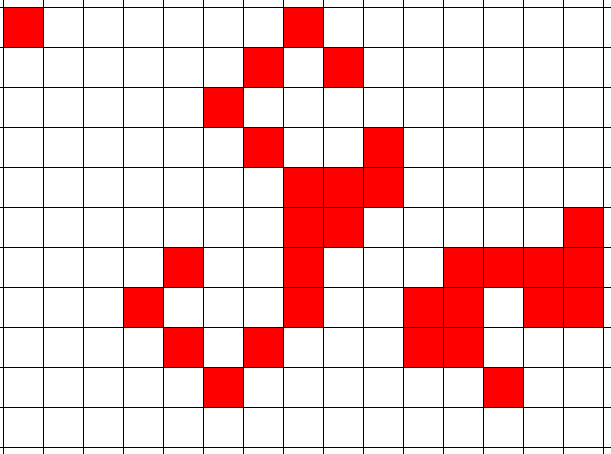
\includegraphics[scale=\myscale,scale=0.3]{screen-life-0}
\end{center} 


%%%%%%%%%%%%%%%%%%%%%%%%%%%%%%%%%%%%%%%%%%%%%%%%%%%%%%%%%%%%%%%%
%%%%%%%%%%%%%%%%%%%%%%%%%%%%%%%%%%%%%%%%%%%%%%%%%%%%%%%%%%%%%%%%

\begin{cours}[Rules of the game of life]
The \emph{game of life}\index{game of life} takes place on a grid. Each square can contain one cell. Starting from an initial configuration, each day cells will be born and others will die depending on the number of its neighbors.

Here are the rules:
\begin{itemize}
  \item For an empty square on day $j$ and having exactly $3$ neighboring cells: a cell is born on day $j+1$.

\myfigure{0.5}{
  \tikzinput{fig-life-0a}
}

  \item If a square containing a cell at day $j$, has either $2$ or $3$ neighboring cells: then the cell continues to live.
  In other cases the cell dies (with $0$ or $1$ neighbors, it dies of isolation, with more than $4$ neighbors, it dies of overpopulation).
  
  \medskip
  
\myfigure{0.5}{
  \tikzinput{fig-life-0b}
}  

   \medskip
    
\end{itemize}

Here is a simple example, the \og{}blinker\fg{}.

\myfigure{0.5}{
  \tikzinput{fig-life-0c}
} 
 
Here is another example (with the number of neighbors written in each case), the first evolution and the evolution of the evolution.

\myfigure{0.5}{
  \tikzinput{fig-life-0d}
} 
\end{cours}



%%%%%%%%%%%%%%%%%%%%%%%%%%%%%%%%%%%%%%%%%%%%%%%%%%%%%%%%%%%%%%%%
% Activity 1
%%%%%%%%%%%%%%%%%%%%%%%%%%%%%%%%%%%%%%%%%%%%%%%%%%%%%%%%%%%%%%%%

\begin{activite}[Display]
\objectifs{Goal: define and display arrays.}

We model the living space of the cells by a double entry table, containing integers, $1$ to indicate the presence of a cell, $0$ otherwise. Here is an example of the \og{}toad\fg{} configuration and its array:

\myfigure{0.6}{
  \tikzinput{fig-life-1}
} 

\begin{enumerate}
  \item 
  \begin{itemize}
    \item Initialize two variables: \ci{n} (the height of the table) and \ci{p} (the width) (for example at $5$ and $8$).
    
    \item Define a two-dimensional table filled with zeros by the command:  
    \mycenterline{\ci{array = [[0 for j in range(p)] for i in range(n)]}}
    
    \item By using instructions of the type \ci{array[i][j] = 1}, fill in the table to define the configurations of the blinker, the toad \ldots
  \end{itemize}
  
  \item Program the display of a given array on the screen. 
  For example, the blinker is displayed as follows:
  
\begin{center}
\ci{00000000}\\
\ci{00000000}\\
\ci{00111000}\\
\ci{00000000}\\
\ci{00000000}
\end{center}

  \emph{Hint.} By default the \ci{print()} function starts a new line on each call (it effectively adds \ci{"\\n"} which is the end of line character). It can be specified not to do this by the option \ci{print("My text",end="")}.
  
\end{enumerate}
\end{activite}



%%%%%%%%%%%%%%%%%%%%%%%%%%%%%%%%%%%%%%%%%%%%%%%%%%%%%%%%%%%%%%%%
% Activity 2
%%%%%%%%%%%%%%%%%%%%%%%%%%%%%%%%%%%%%%%%%%%%%%%%%%%%%%%%%%%%%%%%

\begin{activite}[Graphic display]

\objectifs{Goal: create a graphical display of a cell configuration.}

\begin{center}
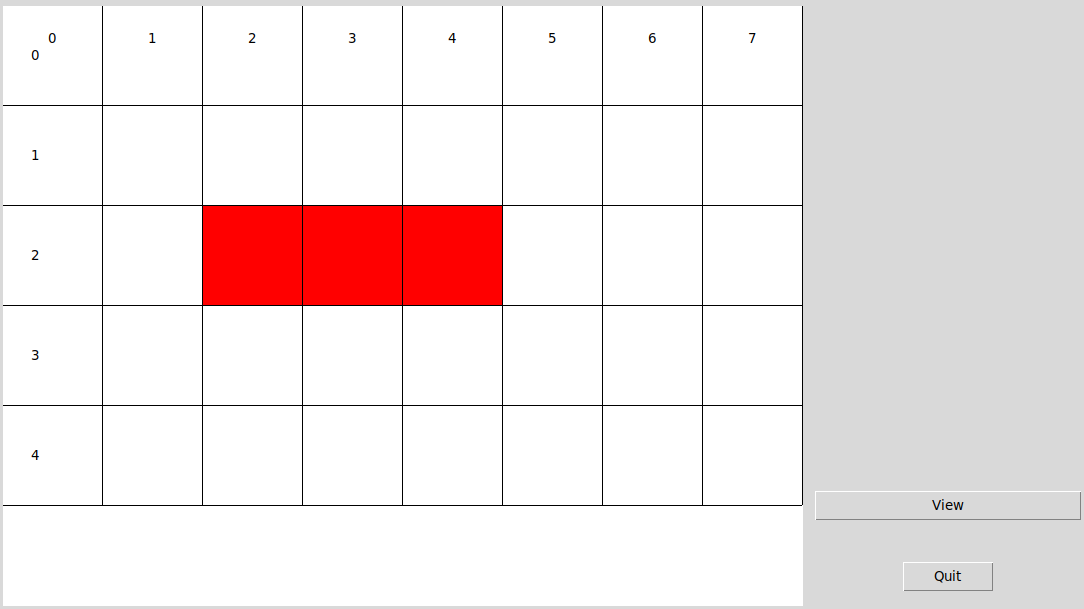
\includegraphics[scale=\myscale,scale=0.3]{screen-life-2-en}
\end{center} 

\begin{enumerate}
  \item Program the creation of a \ci{tkinter} window (see the \og{}Statistics -- Data visualization\fg{} chapter). Write a \ci{draw_grid()} function, without parameters, that displays a blank grid of coordinates. You will need a constant \ci{scale} (for example \ci{scale = 50}) to transform the indices $i$ and $j$ into graphic coordinates $x$ and $y$, depending on the relationship: $x= s \times j$ and $y = s \times i$ ($s$ being the scale).
  
  \textbf{Bonus.} You can also mark the values of the indices $i$ and $j$ at the top and the left to make it easier to read the grid.
  
  \item Build a \ci{draw_array(array)} function that graphically displays the cells from a table. 
  
  \textbf{Bonus.}  Add a \og{}View\fg{} button and a \og{}Quit\fg{} button
(see the \og{}Statistics -- Data visualization\fg{} chapter).  
  
\end{enumerate}
\end{activite}



%%%%%%%%%%%%%%%%%%%%%%%%%%%%%%%%%%%%%%%%%%%%%%%%%%%%%%%%%%%%%%%%
% Activity 3
%%%%%%%%%%%%%%%%%%%%%%%%%%%%%%%%%%%%%%%%%%%%%%%%%%%%%%%%%%%%%%%%

\begin{activite}[Evolution]

\objectifs{Goal: calculate the evolution of a configuration from one day to the next.}

\begin{enumerate}
  \item Program a \ci{number_neighbors(i,j,array)} function that calculates the number of living neighboring cells to the cell $(i,j)$.
  
  \emph{Hints.}
  \begin{itemize}
    \item There is a maximum of $8$ possible neighbors. The easiest way is to test them one by one!
    \item For counting, it is necessary to be very careful with the cells that are placed near an edge (and have less than $8$ possible neighbors).
  \end{itemize}
  
  \item Program an \ci{evolution(array)} function that receives a table as an input and returns a new array corresponding to the situation on the next day, according to the rules of the game of life described at the beginning.
 For example, if the table on the left corresponds to the input, then the output corresponds to the table on the right:

\begin{center}
\begin{minipage}{0.3\textwidth}
\begin{center}
\ci{00000000}\\
\ci{00000000}\\
\ci{00111000}\\
\ci{00000000}\\
\ci{00000000}
\end{center}
\end{minipage} 
 evolves in  
\begin{minipage}{0.3\textwidth}
\begin{center}
\ci{00000000}\\
\ci{00010000}\\
\ci{00010000}\\
\ci{00010000}\\
\ci{00000000}
\end{center}
\end{minipage} 
\end{center}

  \emph{Hints.} To define a new table, use the command:  
      \mycenterline{\ci{new_array = [[0 for j in range(p)] for i in range(n)]}}      
  and then modify the table as desired.

\end{enumerate}
\end{activite}


 

%%%%%%%%%%%%%%%%%%%%%%%%%%%%%%%%%%%%%%%%%%%%%%%%%%%%%%%%%%%%%%%%
% Activity 4
%%%%%%%%%%%%%%%%%%%%%%%%%%%%%%%%%%%%%%%%%%%%%%%%%%%%%%%%%%%%%%%%

\begin{activite}[Iterations]

\objectifs{Goal: complete the graphic program so that the user can define configurations and make them evolve with a simple click.}

\begin{enumerate}
  \item Improve the graphics window to make the user's life easier:
  \begin{itemize}
    \item An \og{}evolve\fg{} button which displays the next evolution with each click.
    \item Buttons to display predefined configurations (in the screenshot below is the configuration \og{}pentadecathlon\fg{}).
  \end{itemize}
  
\begin{center}
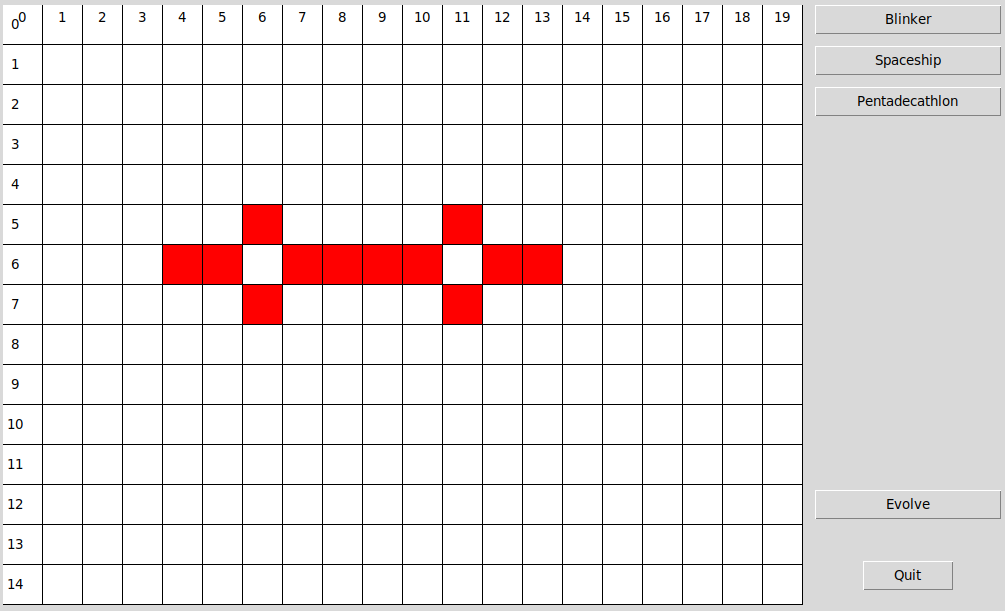
\includegraphics[scale=\myscale,scale=0.3]{screen-life-4a-en}
\end{center}  
  
  \item Perfect your program so that the user can draw the configuration he wants with mouse clicks. Clicking on an extinguished cell turns it on, clicking on an living cell turns it off. 
  You can break this task down into three functions:
  \begin{itemize}
    \item \ci{on_off(i,j)}, which switches the cell $(i,j)$.
    \item \ci{xy_to_ij(x,y)} that converts graphic coordinates $(x,y)$ into integers coordinates $(i,j)$ (use the \ci{scale}  variable and the integer division).
    \item \ci{action_click_mouse(event)} to retrieve the coordinates $(x,y)$ with a mouse click (see course below) and switch the clicked box.
  \end{itemize}   
    
\begin{center}
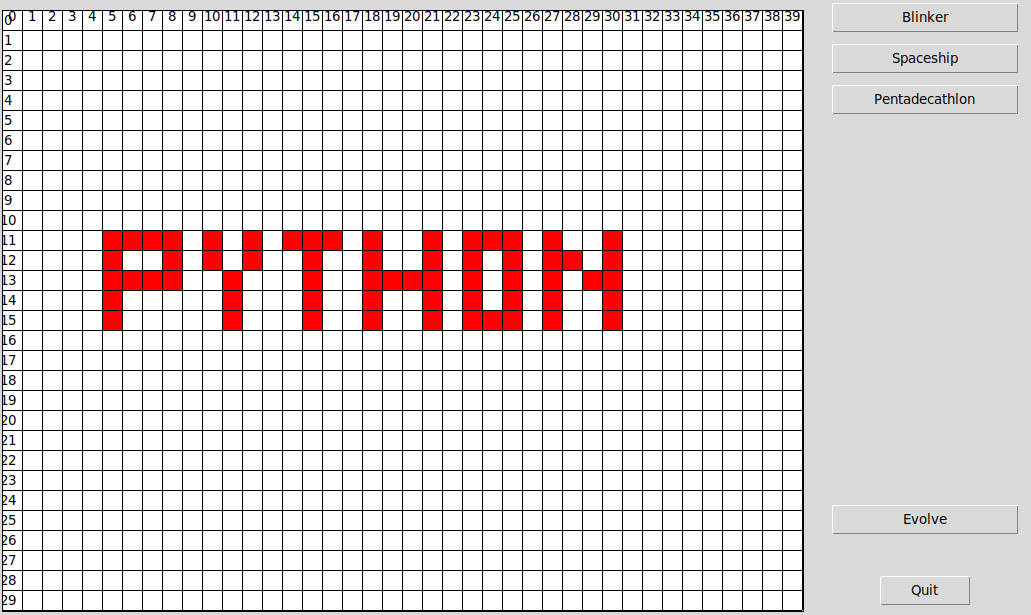
\includegraphics[scale=\myscale,scale=0.3]{screen-life-4b-en}
\end{center}

    
\end{enumerate}
\end{activite} 


\begin{cours}[Mouse click]

\index{tkinter@\ci{tkinter}}
\index{module!tkinter@\ci{tkinter}}
\index{mouse}
\index{click}

Here is a small program that displays a graphic window. Each time the user clicks (with the left mouse button) the program displays a small square (on the window) and displays \og{}Click at $x=\ldots$, $y=\ldots$\fg{} (on the console).

\begin{lstlisting}
from tkinter import *

# Window
root = Tk()
canvas = Canvas(root, width=800, height=600, background="white")
canvas.pack(side=LEFT, padx=5, pady=5)

# Catch mouse click
def action_mouse_click(event):
    canvas.focus_set()
    x = event.x
    y = event.y
    canvas.create_rectangle(x,y,x+10,y+10,fill="red")
    print("Click at x =",x,", y =",y)
    return

# Association click/action
canvas.bind("<Button-1>", action_mouse_click)

# Launch
root.mainloop()
\end{lstlisting}


Here are some explanations:
\begin{itemize}
  \item The creation of the window is usual. The program ends with the launch of the \ci{mainloop()} command.
  
  \item The first key point is to associate a mouse click to an action, that's what this line does: 
\mycenterline{\ci{canvas.bind("<Button-1>", action_mouse_click)}}

Each time the left mouse button is clicked, \Python{} executes the function \ci{action_mouse_click}. (Note that there are no brackets for the call to the function.)

   \item Second key point: the \ci{action_mouse_click} function retrieves the click coordinates and then does two things here: it displays a small rectangle at the click location and prints the $(x,y)$ coordinates to the terminal window.
   
   \item The coordinates $x$ and $y$ are expressed in pixels; $(0,0)$ refers to the upper left corner of the window (the area delimited by \ci{canvas}).
\end{itemize}
\end{cours}



Here are some ideas to go further:
\begin{itemize}
  \item Make sure that the grid automatically adapts to the screen width, i.e. calculate \ci{scale} based on \ci{n} and \ci{p}.
  
  \item Add an intermediate step before evolving: color  a cell that will be born  in green and a cell that will die in black. For this purpose the elements of \ci{array} can take values other than $0$ and $1$.
\end{itemize}

Here are some interesting configurations. 
\myfigure{0.6}{
  \tikzinput{fig-life-4a} \quad 
  \tikzinput{fig-life-4b} 
} 

You will find many more on the Internet but above all have fun discovering new ones!

In particular, find configurations:
\begin{itemize}
  \item which remain fixed over time;
  \item which evolve, then become fixed;
  \item which are periodic (the same configurations come back in loops) with a period of $2$, $3$ or more;
  \item which travel;
  \item which propel cells; 
  \item whose population is increasing indefinitely!
\end{itemize}


\end{document}
